\chapter{提案手法}
\label{ch:proposal}
\begin{figure}[H]
  \begin{center}
    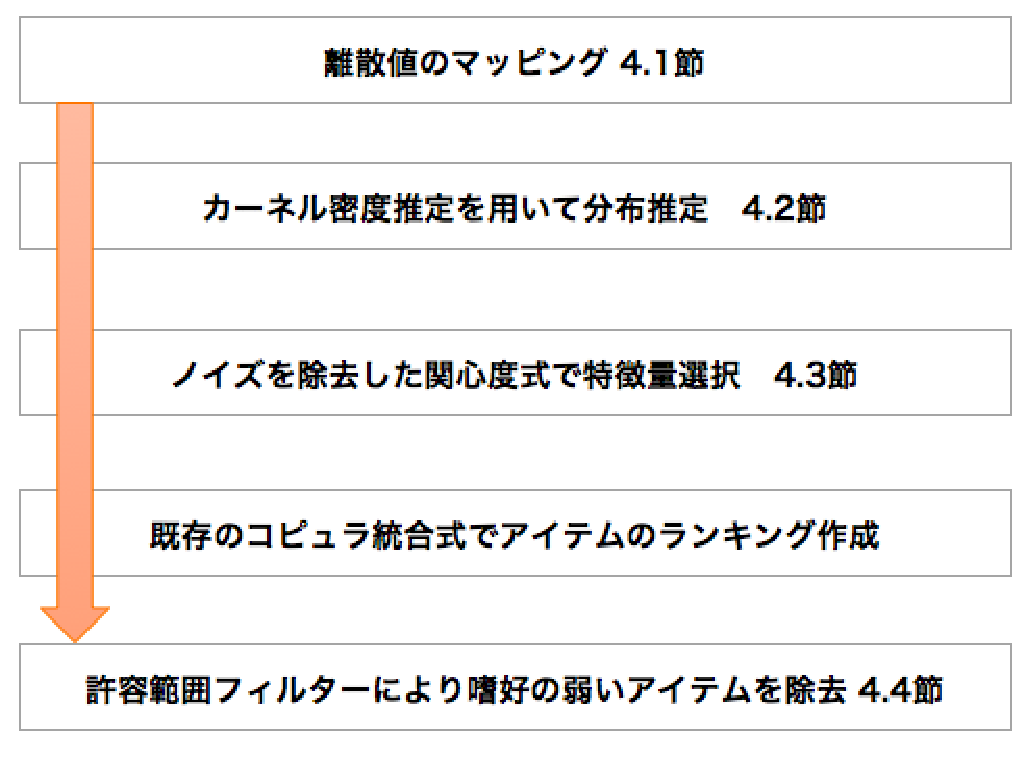
\includegraphics[width=5in]{source/proposal.eps}
  \vspace{1mm}
  \caption{提案手法の処理チャート} %\vspace{-3mm}
  \label{fig:proposal}
  %\vspace{-0.4cm}
  \end{center} 
\end{figure}
\hspace{1em}本提案手法は以下の4つの構成から成っており,鈴木らのシステムでは扱えない離散値特徴量や特異な分布を扱うためのものである.\par
提案手法の処理チャートは図\ref{fig:proposal}である.
\begin{enumerate} 
  \item ユーザの嗜好を反映した離散値特徴量への数値マッピング (\ref{sc:mapping}節)
  \item カーネル密度推定を利用した複雑な分布への対応 (\ref{sc:mix_gaussian}節)
  \item 鈴木らの関心度式からノイズ部分を除去して,離散値特徴量へ対応 (\ref{sc:att_shr}節)
  \item 許容範囲フィルターにより,特徴量値の特定区間にこだわりをもつような特異な嗜好ケースに対応 (\ref{sbsc:tlr}節)
\end{enumerate}
\section{離散値特徴量への数値マッピング}
\label{sc:mapping}
特徴量の累積分布を求めるためには,特徴量を数直線上の実数値にマッピングする
必要がある.
特徴量の累積分布は特徴量に対して単調増加するため,
特徴量が離散値の場合,数値を離散値に割り当てる順番が累積分布の値に影響する.
この際にユーザがもつ,離散値特徴量への嗜好順を考慮すべきである.\par
例えば,喫煙可能か禁煙かを表す離散値特徴量として喫煙値というものを定義し,これに0と1の数値を割り当てる場合を考える.
ユーザが禁煙家の場合は禁煙に1,喫煙可能に0を割り当てるべきなのに対し,ユーザが喫煙家の場合は喫煙可能に1,禁煙に0を割り当てるべきである.\par
このように嗜好順を考慮したマッピングをするために人気度$ppl$を以下のように定義した.
$i$番目の特徴量の離散値$v$に対して,ユーザがもつ人気度$ppl_i(v)$は式(\ref{eq:ppl})で定義される.
\begin{comment}
  \label{eq:popular}
  &like_{User}(x)=\left\{
    \begin{array}{ll}
      1 &(User\hphantom{a}likes\hphantom{a}x) \\
    0 &(otherwise) 
\end{array}\right. & \\
  &S_{User}=\{item|like_{User}(item)==1\}& \\
\end{comment}

\begin{gather*}
  S_{ScoreUser}(i,v)=\{item|score_{i}(item)=v\}\cap S_{User} \\
  S_{ScoreAll}(i,v)=\{item|score_{i}(item)=v\}\cap S_{All} \\
\end{gather*}
\begin{equation}
  \label{eq:ppl}
  ppl_i(v)=\frac{|S_{ScoreUser}(i,v)|}{|S_{ScoreAll}(i,v)|}
\end{equation}\par
$score_{i}(item)$は$item$の特徴量$i$のスコア値を返す関数,$S_{User}$はユーザが選択した$item$集合,$S_{All}$は全$item$集合であることに注意する.
$ppl_i(v)$は$i$番目の特徴量が$v$の$item$集合から,ユーザがどれだけの$item$に関心を示したかを表している.\par
この人気度$ppl$の高い離散値から降順で高い数値を割り当てることで,ユーザの嗜好を考慮して,離散値特徴量に数値を割り当てられることが期待できる.
\section{カーネル密度推定を利用した複雑な分布への対応}
\label{sc:mix_gaussian}
鈴木らのシステム\cite{Suzuki}が特徴量分布の推定に正規分布モデルを用いていたのに対し,本研究ではカーネル密度推定を用いる.
これにより,特徴量の分布が正規分布にならない場合にも対応できることが期待できる.
式(\ref{eq:kde})のパラメータであるカーネル関数式には式(\ref{eq:kernel})を
用いた.
\begin{equation}
\label{eq:kernel}
K(x)=\left\{
\begin{array}{ll}
  tophat(x) & (特徴量xが離散値) \\
  gaussian(x) & (特徴量xが連続値) \\
\end{array} \right.
\end{equation}

\begin{equation}
  \label{eq:tophat}
  tophat(x)=\left\{
  \begin{array}{ll}
    \frac{1}{2} &(-1 \leq x \leq 1) \\
    0 &(otherwise) \\
  \end{array} \right.
\end{equation}

\begin{equation}
  \label{eq:gaussian}
  gaussian(x)=
  \frac{1}{2\sqrt{\pi}\sigma}exp\left(-\frac{{(x-u)}^2}{2{\sigma}^2}\right) \\
\end{equation}

\subsection{バンド幅の決定}
カーネル密度推定式(式(\ref{eq:kde}))のパラメータであるバンド幅$h$の選択には式(\ref{eq:h})のようにカーネル関数$K(x)$の特性に合ったものを用いた.
連続値の場合,最適値の位置を探るための$S_{lct}$と\ref{sbsc:related_bw}の$h_{2}$,$h_{1}$からなる$S_{opt}$から構築した探索集合$S_{Grd}$から$GridSearch$で最適値$h_{G\_opt}$を選択する.
$S_{lct}$は$K(x)$が$gaussian(x)$で累積分布が求まるという条件と,常用対数が負であるという条件を同時に満たす要素の集合である.\\
\begin{equation}
  \label{eq:h}
  h_{opt}=\left\{
    \begin{array}{ll}
  0.1 &(K=tophat)\\
  h_{G\_opt} &(K=gaussian)
\end{array}\right.
\end{equation}

\begin{gather}
\label{eq:kde_lct}
S_{lct}=\{10^{-3},5\cdot 10^{-3},10^{-2},...,5\cdot 10^{-1}\} \\
\label{eq:kde_opt}
S_{opt}=\{silverman,scott\} \\
\label{eq:kde_search}
S_{Grd}=S_{lct}\cup S_{opt}
\end{gather}


\begin{comment}
\begin{flalign}
\label{eq:kde_lct}
&S_{lct}=\{10^{-3},5\cdot 10^{-3},10^{-2},...,5\cdot 10^{-1}\}& \\
\label{eq:kde_opt}
&S_{opt}=\{silverman,scott\}& \\
\label{eq:kde_search}
&S_{Grd}=S_{lct}\cup S_{opt}&
\end{flalign}
\end{comment}
以下に$Gridserach$の概要を載せる.
\begin{enumerate}
  \item 訓練用データ集合$S_{trn}$からこれを$k$分割した各集合$S_{Nscr\_i}$を除いた評価用集合$S_{scr\_i}$を得る.
  \item $S_{Grd}$から,未評価の要素$h$をとりだす.
  \label{itm:grd1}
  \item 式(\ref{eq:score_i_h})のようにして$S_{scored\_i}$で$h$の評価値を求める.
  \item 式(\ref{eq:score_h})のようにして全評価用集合での評価値平均を$h$の評価値とする.
  \label{itm:grd2}
\item (\ref{itm:grd1})から(\ref{itm:grd2})を全$h$に対して行い,$h$の評価値が最大となるものを$h_{G\_opt}$とする.
\end{enumerate}
\begin{eqnarray}
  \label{eq:trn_data}
  S_{scr\_i}&=&S_{trn}\backslash S_{Nsrc\_i} \\
  \label{eq:score_i_h}
  score(h,i)&=&\sum_{x\in S_{scored\_i}}\log f(x) \\
  \label{eq:score_h}
  score(h)&=&\frac{1}{k}\sum_{i=1}^k score(h,i)
\end{eqnarray}
\par
離散値の場合,カーネル関数が$tophat$なので各離散値点で$tophat$が干渉しないようなバンド幅を選択すれば推薦に必要な累積分布を得ることができる.
本研究で用いる離散値は0と1の値をとるため,バンド幅は$0.5$以下になればよい.
よって,離散値のバンド幅には,$0.5$未満で,常用対数が整数であるという条件をみたす実数の最大値である$0.1$を採用した.

\begin{comment}
Set_{int}&=&\{x|\log_{10} x \in \mathbb{Z}\land\\
         && -3 <\log_{10} x < 0\} \nonumber \\
\label{eq:kde_middle}
Set_{middle}&=&\{x| x=middle(y_i,y_{i+1})\}\\
\end{comment}

\section{ノイズを除去した関心度式}
\label{sc:att_shr}
既存の鈴木らの関心度式$Att_i$(式(\ref{eq:Att}))では積分区間が無限区間であり,スコア値の範囲である区間[0,1]以外の計算結果が含まれていた.
しかし,区間[0,1]以外の計算結果をノイズとしたとき,離散値の場合,$tophat$を用いるためノイズが0になる.
よって既存の関心度式で連続値と離散値を比較する場合,ノイズ差を考慮していない問題が生じる.
よって新たな関心度式(式(\ref{eq:new_att}))を$Att_{i\_Shr}$として提案する.
\begin{eqnarray}
     \label{eq:new_att}
     {Att}_{i\_Shr} &=& D_{\mathrm{KL}}(User_i\|ALL_i) \nonumber \\
               &=& (\int_{0}^{1} pdf_{user}(x_{i}) \log \frac{pdf_{user}(x_{i})}{pdf_{all}(x_{i})} \; dx)
 \end{eqnarray}
 \par
 式(\ref{eq:new_att})は既存の算出式$Att$の積分区間を変更し,ノイズが計算結果に含まれないようにしたものである.
 さらに$pdf_{all}(x)\leq pdf_{user}(x)$の部分をより反映させるために鈴木らが用いた$D_{\mathrm{KL}}$のベースを$All_i$から$User_i$へ変更した.区間変更に伴い,値調整のための$log_{1p}$が不要になったためこれを取り除いた.

\section{許容範囲フィルター}
\label{sbsc:tlr}
\begin{table}[H]
  \begin{center} {
    \caption{特異な分布例} \label{tbl:abnormal_role}
    \begin{tabular}{lp{25em}} 
\hline
ROLE番号 & ROLEの説明\\ \hline
ROLE7 & 駅の騒音と徒歩距離を考慮して,駅から適度な距離のホテルがよい.\\
ROLE14 & 同僚と出張で宿泊する.6,000円/人まで会社経費.ホテルはルームチャージ制のため,個人利用であれば,低価格のホテルしか利用できず,相部屋で利用する場合,高価格のホテルまで利用できる.\\
\hline
    \end{tabular}
  }
  \end{center} %\vspace{-8mm}
\end{table}
鈴木らのシステム\cite{Suzuki}はユーザの選択したアイテムを教師データとして構築したコピュラモデルから,推薦対象のアイテムの累積分布を求め,その累積分布の降順で推薦を行うものである.しかし予備調査の結果,表\ref{tbl:abnormal_role}のROLE7やROLE14のような状況において,特徴量の数値が高いがユーザが関心を示していないアイテムが上位に推薦されてしまうという問題が生じため$tlr$の提案を行う.\par
$tlr_i$は特徴量$i$と,ユーザが選択したアイテムの密度分布$pdf_{user}(x)$と,全アイテムの密度分布$pdf_{all}(x)$を考えるとき,式(\ref{eq:tlr})のように定義される.
\begin{equation}
\label{eq:tlr}
tlr_{i}=\{x | pdf_{all,i}(x) \leq pdf_{user,i}(x)\}
\end{equation}
\par
$tlr_i$は,特徴量$i$について全アイテムの$pdf$である$pdf_{all,i}$よりも,ユーザが関心を示したアイテムの$pdf$である$pdf_{user,i}$が上回るような区間であり,ユーザが特に関心を示す特徴量値の範囲を抽出するためのものである.
許容範囲フィルターを特異な分布をとる特徴量$i$の値が,$tlr_{i}$に含まれるアイテムを優先的に選択する手法として定義する.
この手法を用いれば,特定の特徴量値が特定の範囲にあるアイテムに強い嗜好を示すようなケースに対応できることが期待できる.\par
しかし,この許容範囲フィルターを有効にする特徴量をどのようにして選択するかという問題がある.
許容範囲フィルターを有効にする特徴量が多いほど,アイテムが推薦対象から外される可能性が高くなりフィルターが有効に機能しにくくなる.\par
よって,特異な分布をとる特徴量を含むできるだけ小さい特徴量集合で,フィルターを有効にするのが望ましい.
特異な分布をとる特徴量の場合,ユーザはその特徴量に強い関心をもっていることが想定される.
よって,鈴木らの手法を用いて重要次元$S_{emp}$(式(\ref{eq:set_emp}))を抽出して,$S_{emp}$でフィルターを有効にするという手法が候補に上がる.
しかし,関心度が一部の特徴量で拮抗しているため重要な特徴量が外れ値として検出できないような場合に,特定の特徴量が特異な分布をとるにもかかわらずフィルターが有効にならないというケースを考慮して,フィルターを有効にする特徴量集合$S_{fitered}$を(式(\ref{eq:S_filtered}))のように定義する.

\begin{equation}
\label{eq:S_filtered}
S_{filtered}=\left\{
  \begin{array}{ll}
    S_{sorted}(n) &(S_{emp}=\phi)\\
    S_{emp} &(otherwise)\\
  \end{array}\right.
\end{equation}
\par
(式(\ref{eq:S_filtered}))は重要次元$S_{emp}$が要素をもつ場合は$S_{emp}$の特徴量でフィルターを有効にし,$S_{emp}$が空の場合は鈴木らの関心度式で算出した関心度の降順で$n$番目までの特徴量からなる集合$S_{soreted}(n)$の特徴量でフィルターを有効にすることを意味する.
$n$には,評価実験でU字型の分布が確認できた全特徴量を抽出できる整数のうち,最小の値である$n=2$を用いた.\par
この$S_{filtered}$の各特徴量$i$の値が$tlr_i$に含まれるという条件を満たすようなアイテムを優先的に推薦することで,特異な分布をとらない特徴量による影響を抑えつつ許容範囲フィルターを用いて適切な推薦ができることが期待できる.
